%-----------------------------------------------------------------------------------------------------------------------------------------------%
%	The MIT License (MIT)
%
%	Copyright (c) 2019 Jan Küster
%
%	Permission is hereby granted, free of charge, to any person obtaining a copy
%	of this software and associated documentation files (the "Software"), to deal
%	in the Software without restriction, including without limitation the rights
%	to use, copy, modify, merge, publish, distribute, sublicense, and/or sell
%	copies of the Software, and to permit persons to whom the Software is
%	furnished to do so, subject to the following conditions:
%
%	THE SOFTWARE IS PROVIDED "AS IS", WITHOUT WARRANTY OF ANY KIND, EXPRESS OR
%	IMPLIED, INCLUDING BUT NOT LIMITED TO THE WARRANTIES OF MERCHANTABILITY,
%	FITNESS FOR A PARTICULAR PURPOSE AND NONINFRINGEMENT. IN NO EVENT SHALL THE
%	AUTHORS OR COPYRIGHT HOLDERS BE LIABLE FOR ANY CLAIM, DAMAGES OR OTHER
%	LIABILITY, WHETHER IN AN ACTION OF CONTRACT, TORT OR OTHERWISE, ARISING FROM,
%	OUT OF OR IN CONNECTION WITH THE SOFTWARE OR THE USE OR OTHER DEALINGS IN
%	THE SOFTWARE.
%
%
%-----------------------------------------------------------------------------------------------------------------------------------------------%


%============================================================================%
%
%	DOCUMENT DEFINITION
%
%============================================================================%

%we use article class because we want to fully customize the page and don't use a cv template
\documentclass[10pt,A4]{article}


%----------------------------------------------------------------------------------------
%	ENCODING
%----------------------------------------------------------------------------------------

% we use utf8 since we want to build from any machine
\usepackage[utf8]{inputenc}

%----------------------------------------------------------------------------------------
%	LOGIC
%----------------------------------------------------------------------------------------

% provides \isempty test
\usepackage{xstring, xifthen}

%----------------------------------------------------------------------------------------
%	FONT BASICS
%----------------------------------------------------------------------------------------

% some tex-live fonts - choose your own

%\usepackage[defaultsans]{droidsans}
%\usepackage[default]{comfortaa}
%\usepackage{cmbright}
\usepackage[default]{raleway}
\usepackage{fontawesome}
\usepackage{enumitem}
\setlist{nosep}
%\usepackage{fetamont}
%\usepackage[default]{gillius}
%\usepackage[light,math]{iwona}
%\usepackage[thin]{roboto}

% set font default
\renewcommand*\familydefault{\sfdefault}
\usepackage[T1]{fontenc}

% more font size definitions
\usepackage{moresize}

%----------------------------------------------------------------------------------------
%	FONT AWESOME ICONS
%----------------------------------------------------------------------------------------

% include the fontawesome icon set
\usepackage{fontawesome}

% use to vertically center content
% credits to: http://tex.stackexchange.com/questions/7219/how-to-vertically-center-two-images-next-to-each-other
\newcommand{\vcenteredinclude}[1]{\begingroup
\setbox0=\hbox{\includegraphics{#1}}%
\parbox{\wd0}{\box0}\endgroup}

% use to vertically center content
% credits to: http://tex.stackexchange.com/questions/7219/how-to-vertically-center-two-images-next-to-each-other
\newcommand*{\vcenteredhbox}[1]{\begingroup
\setbox0=\hbox{#1}\parbox{\wd0}{\box0}\endgroup}

% icon shortcut
\newcommand{\icon}[3] {
	\makebox(#2, #2){\textcolor{maincol}{\csname fa#1\endcsname}}
}

% icon with text shortcut
\newcommand{\icontext}[4]{
	\vcenteredhbox{\icon{#1}{#2}{#3}}  \hspace{2pt}  \parbox{0.9\mpwidth}{\textcolor{#4}{#3}}
}

% icon with website url
\newcommand{\iconhref}[5]{
    \vcenteredhbox{\icon{#1}{#2}{#5}}  \hspace{2pt} \href{#4}{\textcolor{#5}{#3}}
}

% icon with email link
\newcommand{\iconemail}[5]{
    \vcenteredhbox{\icon{#1}{#2}{#5}}  \hspace{2pt} \href{mailto:#4}{\textcolor{#5}{#3}}
}

%----------------------------------------------------------------------------------------
%	PAGE LAYOUT  DEFINITIONS
%----------------------------------------------------------------------------------------

% page outer frames (debug-only)
% \usepackage{showframe}

% we use paracol to display breakable two columns
\usepackage{paracol}

% define page styles using geometry
\usepackage[a4paper]{geometry}

% remove all possible margins
\geometry{top=1cm, bottom=1cm, left=1cm, right=1cm}

\usepackage{fancyhdr}
\pagestyle{empty}

% space between header and content
\setlength{\headheight}{0pt}

% indentation is zero
\setlength{\parindent}{0mm}

%----------------------------------------------------------------------------------------
%	TABLE /ARRAY DEFINITIONS
%----------------------------------------------------------------------------------------

% extended aligning of tabular cells
\usepackage{array}

% custom column right-align with fixed width
% use like p{size} but via x{size}
\newcolumntype{x}[1]{%
>{\raggedleft\hspace{0pt}}p{#1}}%


%----------------------------------------------------------------------------------------
%	GRAPHICS DEFINITIONS
%----------------------------------------------------------------------------------------

%for header image
\usepackage{graphicx}

% use this for floating figures
% \usepackage{wrapfig}
% \usepackage{float}
% \floatstyle{boxed}
% \restylefloat{figure}

%for drawing graphics
\usepackage{tikz}
\usetikzlibrary{shapes, backgrounds,mindmap, trees}

%----------------------------------------------------------------------------------------
%	Color DEFINITIONS
%----------------------------------------------------------------------------------------
\usepackage{transparent}
\usepackage{color}

% primary color
\definecolor{maincol}{RGB}{ 225, 0, 0 }

% accent color, secondary
\definecolor{accentcol}{RGB}{ 250, 150, 10 }

% dark color
\definecolor{darkcol}{RGB}{ 70, 70, 70 }

% light color
\definecolor{lightcol}{RGB}{245,245,245}


% Package for links, must be the last package used
\usepackage[hidelinks]{hyperref}

% returns minipage width minus two times \fboxsep
% to keep padding included in width calculations
% can also be used for other boxes / environments
\newcommand{\mpwidth}{\linewidth-\fboxsep-\fboxsep}


%============================================================================%
%
%	CV COMMANDS
%
%============================================================================%

%----------------------------------------------------------------------------------------
%	 EXT Link
%----------------------------------------------------------------------------------------

\newcommand{\extLink}[2]{
	\textcolor{maincol}{\href{#1}{#2}}
}

\newcommand{\extLinkIcon}[2]{
	\textcolor{maincol}{\href{#1}{#2 \,\scriptsize{\faExternalLink} }}
}
%----------------------------------------------------------------------------------------
%	 CV LIST
%----------------------------------------------------------------------------------------

% renders a standard latex list but abstracts away the environment definition (begin/end)
\newcommand{\cvlist}[1] {
	\begin{itemize}\small{#1}\end{itemize}
}

%----------------------------------------------------------------------------------------
%	 CV TEXT
%----------------------------------------------------------------------------------------

% base class to wrap any text based stuff here. Renders like a paragraph.
% Allows complex commands to be passed, too.
% param 1: *any
\newcommand{\cvtext}[1] {
	\begin{tabular*}{1\mpwidth}{p{0.98\mpwidth}}
		\parbox{1\mpwidth}{#1}
	\end{tabular*}
}

%----------------------------------------------------------------------------------------
%	CV SECTION
%----------------------------------------------------------------------------------------

% Renders a a CV section headline with a nice underline in main color.
% param 1: section title
\newcommand{\cvsection}[1] {
	\vspace{14pt}
	\cvtext{
		\textbf{\LARGE{\textcolor{darkcol}{\uppercase{#1}}}}\\[-4pt]
		\textcolor{maincol}{ \rule{0.1\textwidth}{2pt} } \\
	}
}

\newcommand{\cvsectionsmall}[1] {
	\vspace{14pt}
	\cvtext{
		\textbf{\fontsize{14pt}{17pt}\selectfont{\textcolor{darkcol}{\uppercase{#1}}}}\\[-4pt]
		\textcolor{maincol}{ \rule{0.1\textwidth}{2pt} } \\
	}
}

%----------------------------------------------------------------------------------------
%	META SKILL
%----------------------------------------------------------------------------------------

% Renders a progress-bar to indicate a certain skill in percent.
% param 1: name of the skill / tech / etc.
% param 2: level (for example in years)
% param 3: percent, values range from 0 to 1
\newcommand{\cvskill}[3] {
	\begin{tabular*}{1\mpwidth}{p{0.72\mpwidth}  r}
 		\textcolor{black}{\textbf{#1}} & \textcolor{maincol}{#2}\\
	\end{tabular*}%

	\hspace{4pt}
	\begin{tikzpicture}[scale=1,rounded corners=2pt,very thin]
		\fill [lightcol] (0,0) rectangle (1\mpwidth, 0.15);
		\fill [maincol] (0,0) rectangle (#3\mpwidth, 0.15);
  	\end{tikzpicture}%
}


%----------------------------------------------------------------------------------------
%	 CV EVENT
%----------------------------------------------------------------------------------------

% Renders a table and a paragraph (cvtext) wrapped in a parbox (to ensure minimum content
% is glued together when a pagebreak appears).
% Additional Information can be passed in text or list form (or other environments).
% the work you did
% param 1: time-frame i.e. Sep 14 - Jan 15 etc.
% param 2:	 event name (job position etc.)
% param 3: Customer, Employer, Industry
% param 4: Short description
% param 5: work done (optional)
% param 6: technologies include (optional)
% param 7: achievements (optional)
\newcommand{\cvevent}[8] {

	% we wrap this part in a parbox, so title and description are not separated on a pagebreak
	% if you need more control on page breaks, remove the parbox
	\parbox{\mpwidth}{
		\begin{tabular*}{1\mpwidth}{p{0.72\mpwidth}  r}
	 		\textcolor{black}{\textbf{#2}} & \colorbox{maincol}{\makebox[0.28\mpwidth]{\textcolor{white}{#1}}} \\
			\textcolor{maincol}{\textbf{#3}} \ifthenelse{\isempty{#4}}{}{\textcolor{maincol}{\emph{- #4}}}  & \\
		\end{tabular*}\\[8pt]

		\ifthenelse{\isempty{#5}}{}{
			\cvtext{#5}\\
		}
	}

	\ifthenelse{\isempty{#6}}{}{
		\vspace{2pt}
		{#6}
	}

	\ifthenelse{\isempty{#7}}{}{
		\vspace{2pt}
		\cvtext{\textbf{Technologies include:}}\\
		{#7}
	}

	\ifthenelse{\isempty{#8}}{}{
		\vspace{2pt}
		\cvtext{\textbf{Achievements include:}}\\
		{#8}
	}
	\vspace{14pt}
}

%----------------------------------------------------------------------------------------
%	 CV META EVENT
%----------------------------------------------------------------------------------------

% Renders a CV event on the sidebar
% param 1: title
% param 2: subtitle (optional)
% param 3: customer, employer, etc,. (optional)
\newcommand{\cvmetaevent}[4] {
	\textcolor{maincol} {\cvtext{\textbf{\begin{flushleft}#1\end{flushleft}}}}
	\ifthenelse{\isempty{#2}}{}{
	\textcolor{darkcol} {\cvtext{\textbf{#2}} }
	}
	\ifthenelse{\isempty{#3}}{}{
		\cvtext{{ \textcolor{darkcol} {#3} }}\\
	}
}

%============================================================================%
%
%
%
%	DOCUMENT CONTENT
%
%
%
%============================================================================%
\begin{document}
\columnratio{0.8}
\setlength{\columnsep}{2.2em}
\setlength{\columnseprule}{2pt}
\colseprulecolor{lightcol}
\begin{paracol}{2}
\begin{leftcolumn}
%---------------------------------------------------------------------------------------
%	TITLE  HEADER
%----------------------------------------------------------------------------------------
\begin{minipage}[c][3.5cm][c]{1\mpwidth}
	\begin {center}
		\HUGE{ \textbf{ \textcolor{black}{ \uppercase{ Paolo Tagliani } } } } \\[-24pt]
		\textcolor{black}{ \rule{0.1\textwidth}{1.25pt} } \\[4pt]
		\large{ \textcolor{black} {Senior Software Engineer} }
	\end {center}
\end{minipage}

%---------------------------------------------------------------------------------------
%	PROFILE
%----------------------------------------------------------------------------------------
\cvtext{
	I am an experienced Software Engineer and team lead, specialized in full-stack application development, software architecture and technical leadership.\\
	My main goal is delivering good products while learning and improving my skills. \\
	I thrive in remote work settings, having worked remotely since 2015, and I'm a dedicated team player who loves to learn and collaborate.\\
}

%---------------------------------------------------------------------------------------
%	WORK EXPERIENCE
%----------------------------------------------------------------------------------------
\cvsection{WORK EXPERIENCE}

\cvevent
	{Oct 2022 - Present}
	{Senior Full-Stack Software Engineer And Tech Lead}
	{\extLinkIcon{https://www.portchain.com/}{Portchain}}
	{ Copenhagen(DK) - Remote}
	{\begin{itemize}
        \item Led the development of Portchain Connect Alignment Tools, collaborating closely with the product team to implement vertical features.
        \item Coordinated and led a data model migration project that streamlined data processes and enhanced data integrity.
        \item Managed and mentored a team of 5 developers, fostering a collaborative and innovative work environment.
        \item \textbf{Stack}: Node, Express, Typescript, Python, PostgreSQL, PostGIS, Docker, AWS
    \end{itemize}}
	{}
	{}
	{}

\cvevent
	{Aug 2019 - Jun 2022}
	{Full-Stack Software Engineer}
	{Contractor}
	{European Union - Hybrid Remote}
	{\begin{itemize}
        \item Delivered comprehensive product development services for various clients, resulting in successful project completions.
        \item Built scalable enterprise solutions. Demonstrated proficiency in a wide range of technologies, including Swift, Objective-C, C, Go, Python, AWS, Docker, Linux Programming, and Bash, selecting the most appropriate tools based on project requirements.
        \item Implemented DevOps practices to enhance system reliability and streamline deployment processes.
  \end{itemize}}
	{}
	{}
	{}
	{}
	{}

\cvevent
	{Jul 2015 - Jul 2019}
	{Mobile / Full-Stack Software Engineer}
	{\extLinkIcon{https://mobilejazz.com/}{MobileJazz}}
	{Barcelona (ES) - Full Remote}
	{\begin{itemize}
		\item Technical and managerial consultancy for US and European clients.
		\item Worked in several teams: iOS developer in the mobile team, NodeJS developer in the backend, and frontend developer in the web team.
		\item Responsible for DevOps, automation, and custom build solutions in each team.
		\item \textbf{Stack}: Swift, Objective-C, NodeJS, NestJS, Angular, Docker, AWS
	\end{itemize}}
	{}
	{}
	{}
	{}
	{}

  \cvtext{For previous experiences, please refer to my \extLink{https://www.linkedin.com/in/paolo-tagliani-51248117/}{LinkedIn profile}.}

	\vspace{-8pt}


%---------------------------------------------------------------------------------------
%	SKILLS
%----------------------------------------------------------------------------------------
\cvsection{SKILLS}

\begin{tabular*}{1\mpwidth}{p{1\mpwidth}  r}
	\textbf{Programming Languages}\\
	\textcolor{maincol}{\textit{Expert}}: Typescript, Swift, Objective-C/C++ \\
	\textcolor{maincol}{\textit{Advanced}}: C, C++, Javascript, Python,\\
	\textcolor{maincol}{\textit{Familiar}}: Ruby, Go \\
	\\
	\textbf{Frameworks/Libraries}: NodeJS, NestJS, ExpressJS, Angular, React, Cocoa, Cocoa Touch \\
	\textbf{Databases}: PostgreSQL, SQLite, MySQL, MongoDB, Elastic Search \\
	\textbf{Automation}: GitHub Actions, Gitlab CI/CD Pipelines, Travis CI \\
	\textbf{Containerization technologies}: Docker, Docker Compose, Kubernetes \\
  \textbf{AWS}: S3, Lambda, IoT, SNS, ECS, ECR \\
\end{tabular*}


% hotfixes to create fake-space to ensure the whole height is used
% \mbox{}
% \vfill
% \mbox{}
% \vfill
% \mbox{}
% \vfill
% \mbox{}
\end{leftcolumn}
\begin{rightcolumn}
%---------------------------------------------------------------------------------------
%	META IMAGE
%----------------------------------------------------------------------------------------
\vfill \vspace*{160pt}
% 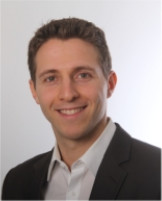
\includegraphics[width=\linewidth]{untitled.jpg}	%trimming relative to image size

%---------------------------------------------------------------------------------------
%	META CONTACT
%----------------------------------------------------------------------------------------
\cvsectionsmall{CONTACT}

\begin{small}
\icontext{MapMarker}{12}{Via Tormini 74/O, Gavardo (BS), Italy}{black}\\[2pt]
\icontext{MobilePhone}{12}{+39 329 2783809}{black}\\[2pt]
\iconemail{Envelope}{12}{pablosproject@gmail.com}{pablosproject@gmail.com}{black}\\[2pt]
\iconhref{Globe}{12}{pablosproject.com}{https://www.pablosproject.com}{black}\\[2pt]
\iconhref{Github}{12}{github.com/pablosproject}{https://github.com/pablosproject}{black}\\[2pt]
\iconhref{Linkedin}{12}{linkedin.com/in/paolo-tagliani}{https://www.linkedin.com/in/paolo-tagliani-51248117}{black}\\[2pt]
\end{small}

%---------------------------------------------------------------------------------------
%	LANGUAGES
%----------------------------------------------------------------------------------------
\cvsectionsmall{LANGUAGES}
\cvlist{
	\item Italian (mother tongue)
	\item English
	\item Spanish
	\item Catalan
}

%---------------------------------------------------------------------------------------
%	EDUCATION
%----------------------------------------------------------------------------------------
\cvsectionsmall{EDUCATION}

\begin{small}
\cvmetaevent
{2010 - 2013}
{Master's Degree in Computer Science}
{University of Brescia}
{}
\cvmetaevent
{2011 - 2012}
{Exchange student in Computer Science}
{LaSalle Barcelona, Ramon Llull University}
{}
\cvmetaevent
{2006 - 2012}
{Bachelor's Degree in Computer Science}
{University of Brescia}
{}
\end{small}

%---------------------------------------------------------------------------------------
%	Projects
%----------------------------------------------------------------------------------------
\cvsectionsmall{Achievements}\\
\begin{small}
\cvtext{
	• US Patent \extLink{https://patents.google.com/patent/US11093747B2/en?oq=US11093747B2}{Hazard Recognition} \\
	• Founder of \extLink{http://pragmamark.org/}{PragmaMark} \\
	• Mentor at \extLink{http://www.coderdojobrescia.it/}{CoderDojo Brescia}
}
\end{small}

\vfill

\end{rightcolumn}
\end{paracol}
\end{document}
